\documentclass[11pt,a4paper]{article}

\usepackage{fullpage}
\usepackage[margin=1in]{geometry}
\usepackage[utf8]{inputenc}
\usepackage{amsmath}

\usepackage{graphicx}
\graphicspath{ {images/} }

\usepackage[colorlinks = true,
            linkcolor = blue,
            urlcolor  = blue,
            citecolor = blue,
            anchorcolor = blue]{hyperref}

\begin{document}

\title{COSC3500 \\ 2D Orbital Simulation Report}
\author{Maxwell Bo (43926871)}
\date{August 17, 2018}
\maketitle

% Description of problem - readable and covers all salient points - /2
\subsection*{Description}
The task was to create a stock-standard, 2-dimensional gravitational $n$-body simulator. 
All bodies were to be assumed to be point masses. The simulation was to be accurate, maintaining a constant total energy, and exhibiting phenomena such as apsidal precession. 
The simulation was to accept arguments specifying the granularity of the simulation (number of time steps, number of instances of data export), and a file specifiying masses and their initial positions and velocities. 
The simulation was to produce its output as fast as possible, with minimal slowdown with an increasing $n$ number of bodies. 

The simulator did not need to handle collisions between bodies.
The MS1 simulator was to be free of OpenMP multiprocessing, which would be implemented in preparation for the MS2 submission.

% Description of implementation - is coherent and has sufficient depth and detail - /5
\subsection*{Implementation}

At a high-level, the initial naive simulator:

\begin{enumerate}
    \item Parsed input parameters and files
    \item Constructed \texttt{Body} class instances, representing each point mass
    \item Packed the \texttt{Body}s into a \texttt{std::vector<Body>}, to maximize cache locality
    \item Calculated forces between all pairwise combinations of $n$-bodies ($O(n^2)$)
    \item Performed Euler's method to derive new velocities and positions
    \item Output all necessary data
    \item \texttt{GOTO 4}
\end{enumerate}

By using a Quadtree, (`a tree datastructure in which each internal node has exactly four children') and the \textit{Barnes-Hut} algorithm\cite{barnes86a}, the total cost of force calculation could be reduced to $O(n \log n)$, by grouping close-together bodies and approximating forces between the singular grouped pseudo-body, and distant bodies. New Quadtrees were constructed on each seperate simulation step.

Dehen and Read note that the Euler method `performs very poorly in practice', further noting that `errors are proportional to $\Delta t^2$'. They contrast it with the second-order \textit{Leapfrog} symplectic integrator, which is `heavily used in collisionless N-body applications'.\cite{dehen11a}

\textit{Leapfrog} can be expressed many in forms\cite{Skeel1993} including a synchronised form:

\begin{align*}
x_{i}&=x_{i-1}+v_{i-1/2}\,\Delta t\\
a_{i}&=F(x_{i})\\
v_{i+1/2}&=v_{i-1/2}+a_{i}\,\Delta t\\
\end{align*}

which only requires a single acceleration calculation per every two half timesteps (the timestep $\Delta t$ must be constant to maintain stability), and a `kick-drift-kick' form

\begin{align*}
v_{i+1/2}&=v_{i}+a_{i}{\frac {\Delta t}{2}}\\
x_{i+1}&=x_{i}+v_{i+1/2}\Delta t\\
v_{i+1}&=v_{i+1/2}+a_{i+1}{\frac {\Delta t}{2}}
\end{align*}

that is stable with variable timstepping, but incurs an additional acceleration calculation per every two half timesteps.

The synchronised form was implemented, but attempts to implement the kick-drift-kick form, and variable timestepping, were left unfinished.

Thus, the final implementation:

\begin{enumerate}
    \item Parsed input parameters and files
    \item Constructed \texttt{Body} class instances, representing each point mass
    \item Packed the \texttt{Body}s into a \texttt{std::vector<Body>}, to maximize cache locality
    \item Inserted all \texttt{Body}s into a fresh \texttt{QuadTree} on full timesteps, traversing the \texttt{QuadTree} with every \texttt{Body} to calculate forces ($O(n \log n)$)
    \item Performed the appropriate \textit{Leapfrog} step to derive new velocities \textit{or} positions
    \item Output all necessary data
    \item \texttt{GOTO 4}
\end{enumerate}

% Why do you believe it is correct - /3
\subsection*{Correctness}

I personally believe that the simulation is relatively accurate. By visualising the results with \texttt{matplotlib}, we see something that resembles an $n$-body simulator. The total energy is flat, observing coefficients of variation as low as 0.001\%. Euler's method consistently demonstrated coefficients of variation three times higher than that of \textit{Leapfrog}. Due to recommendations by literature, and observed data, the use of Euler's method was gradually phased out during my testing to speed up the process.

\textit{Barnes-Hut} caused a significant increase in observed coefficient of variation, averaging 0.08\% across multiple runs. Furthermore, total energy was observed to step up and down at varying intervals\ref{fig:anomaly}. I suspect that this was because certain force calculations were causing groups of bodies to be approximated as a single pseudobody, after other had strayed too far from the pseudobody's quadtree's node's centre of mass.

When bodies are in close proxmity, anomalous total energies are observed\ref{fig:anomaly}. Furthermore, simulations with higher numbers of bodies produce more random low energy outliers (likely due to a greater number of close encounters). There seems to be no signficant difference between Euler method and \textit{Leapfrog}, with respect to observation of anomalies.


\begin{figure}[b]
\caption{Observed energy anomaly while bodies in close proxmity - Leapfrog}
\centering
\label{fig:anomaly}
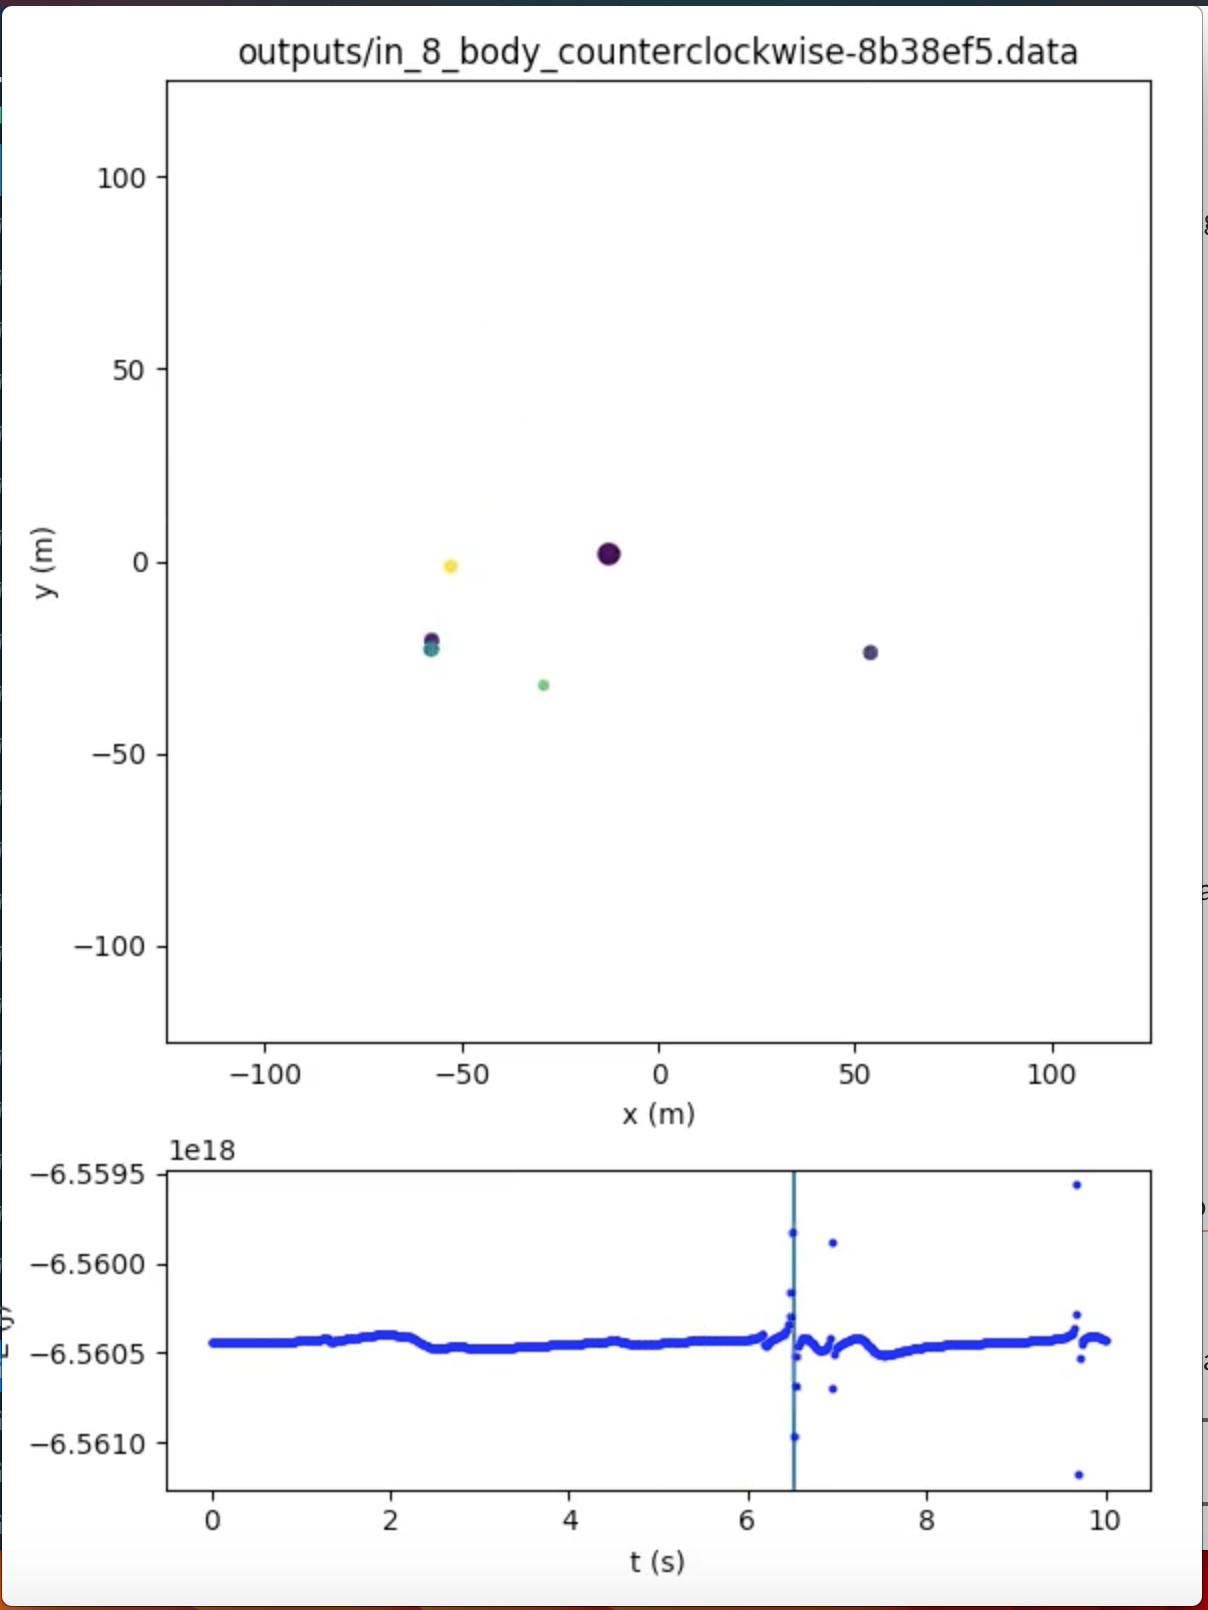
\includegraphics[width=\textwidth]{energy_anomaly}
\end{figure} 

\begin{figure}[b]
\caption{Barnes-Hut energy variation - Leapfrog}
\centering
\label{fig:barnes_hut}
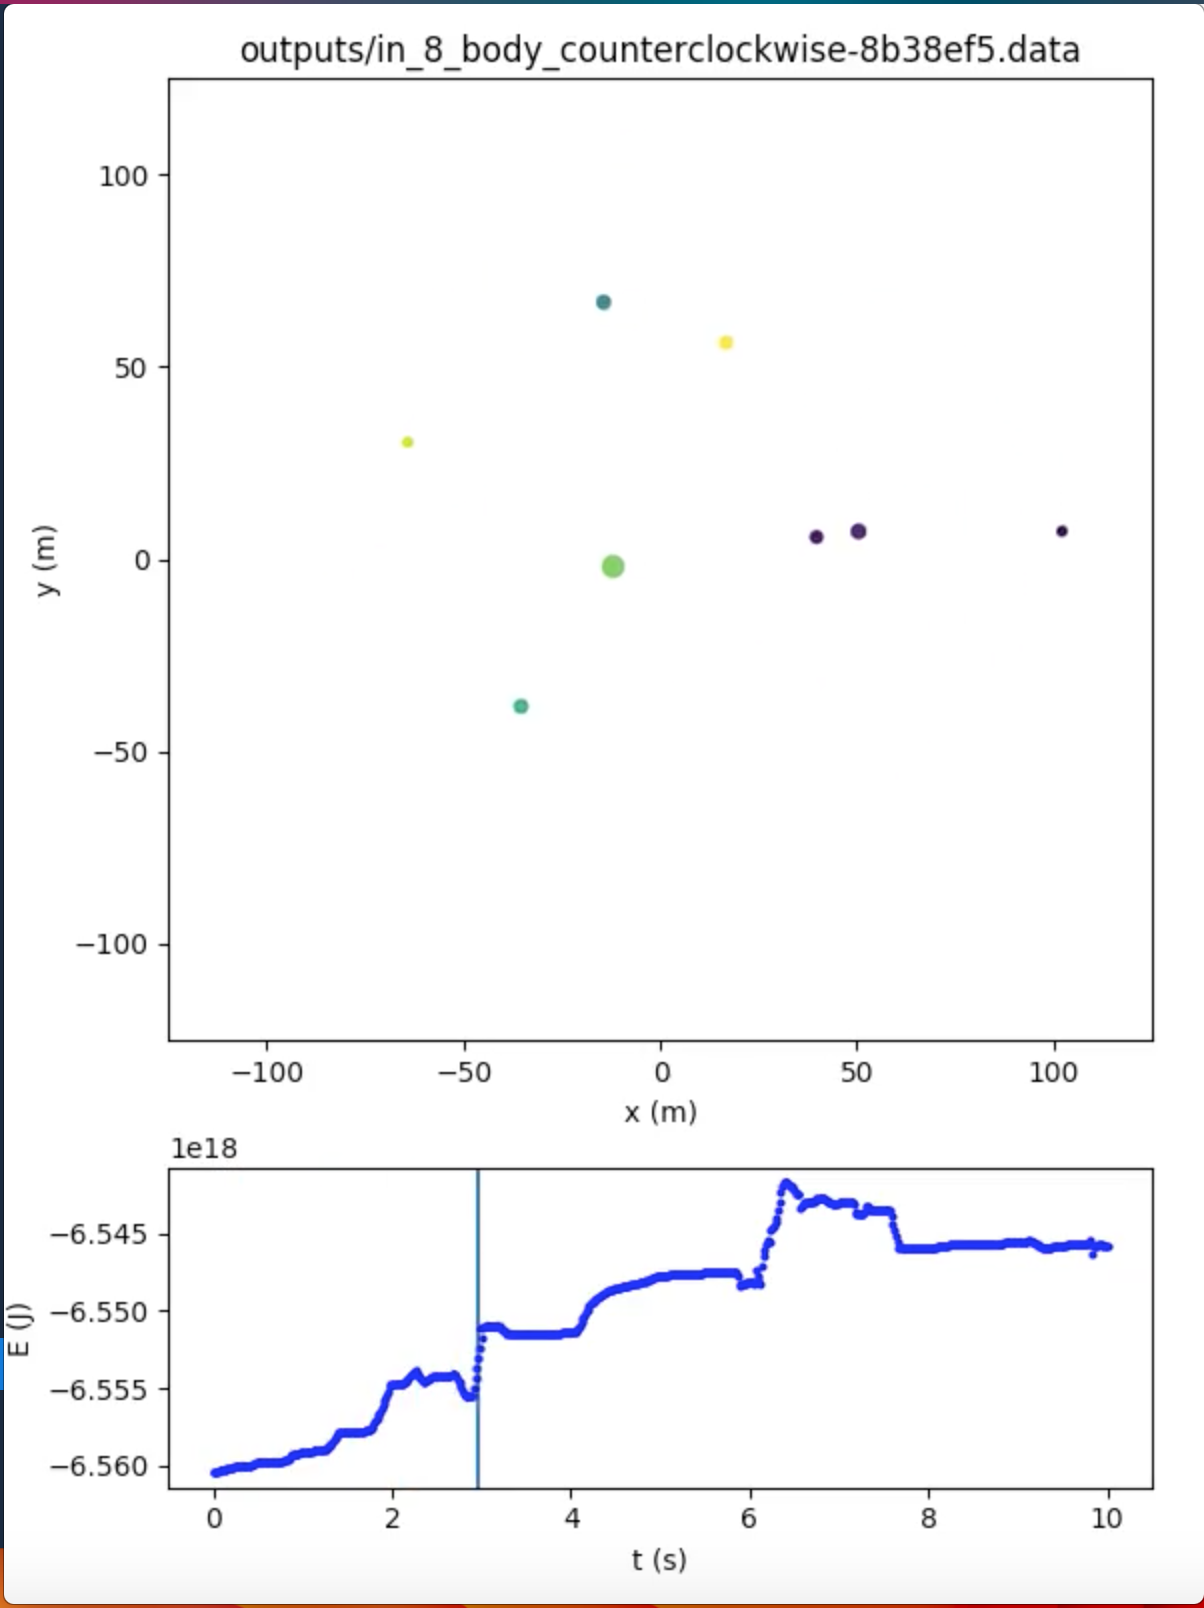
\includegraphics[width=\textwidth]{barnes_hut}
\end{figure} 

% Scaling or other performance discussion - /2
\subsection*{Performance \& Scaling}

Henceforth, the use of the `recognizable' refers to eyeballing the output data, and making no significant effort to investigate the data more rigorously.

The \textit{Barnes-Hut} algorithm appeared to be dominated by its constant factor.\ref{fig:performance} Generating input files with a high number of bodies that did not cause 'spontaneous combustion' (where bodies would fly away from each other in every direction), and unconstrained Quadtree growth (where bodies achieve escape velocity, rapidly expanding the size of the tree and causing a collapse in simulation accuracy) proved difficult. Further testing on \texttt{goliath} is needed to discover the $n$ that causes \textit{Barnes-Hut} to be more performant than the brute-force approach.

Strangely, $n = 16$ with \textit{Barnes-Hut} enabled took longer than expected, when compared to $n \in \{ 4, 8, 12 \}$. Further investigation is required.
\begin{figure}[b]
\caption{Scaling characteristics}
\centering
\label{fig:performance}
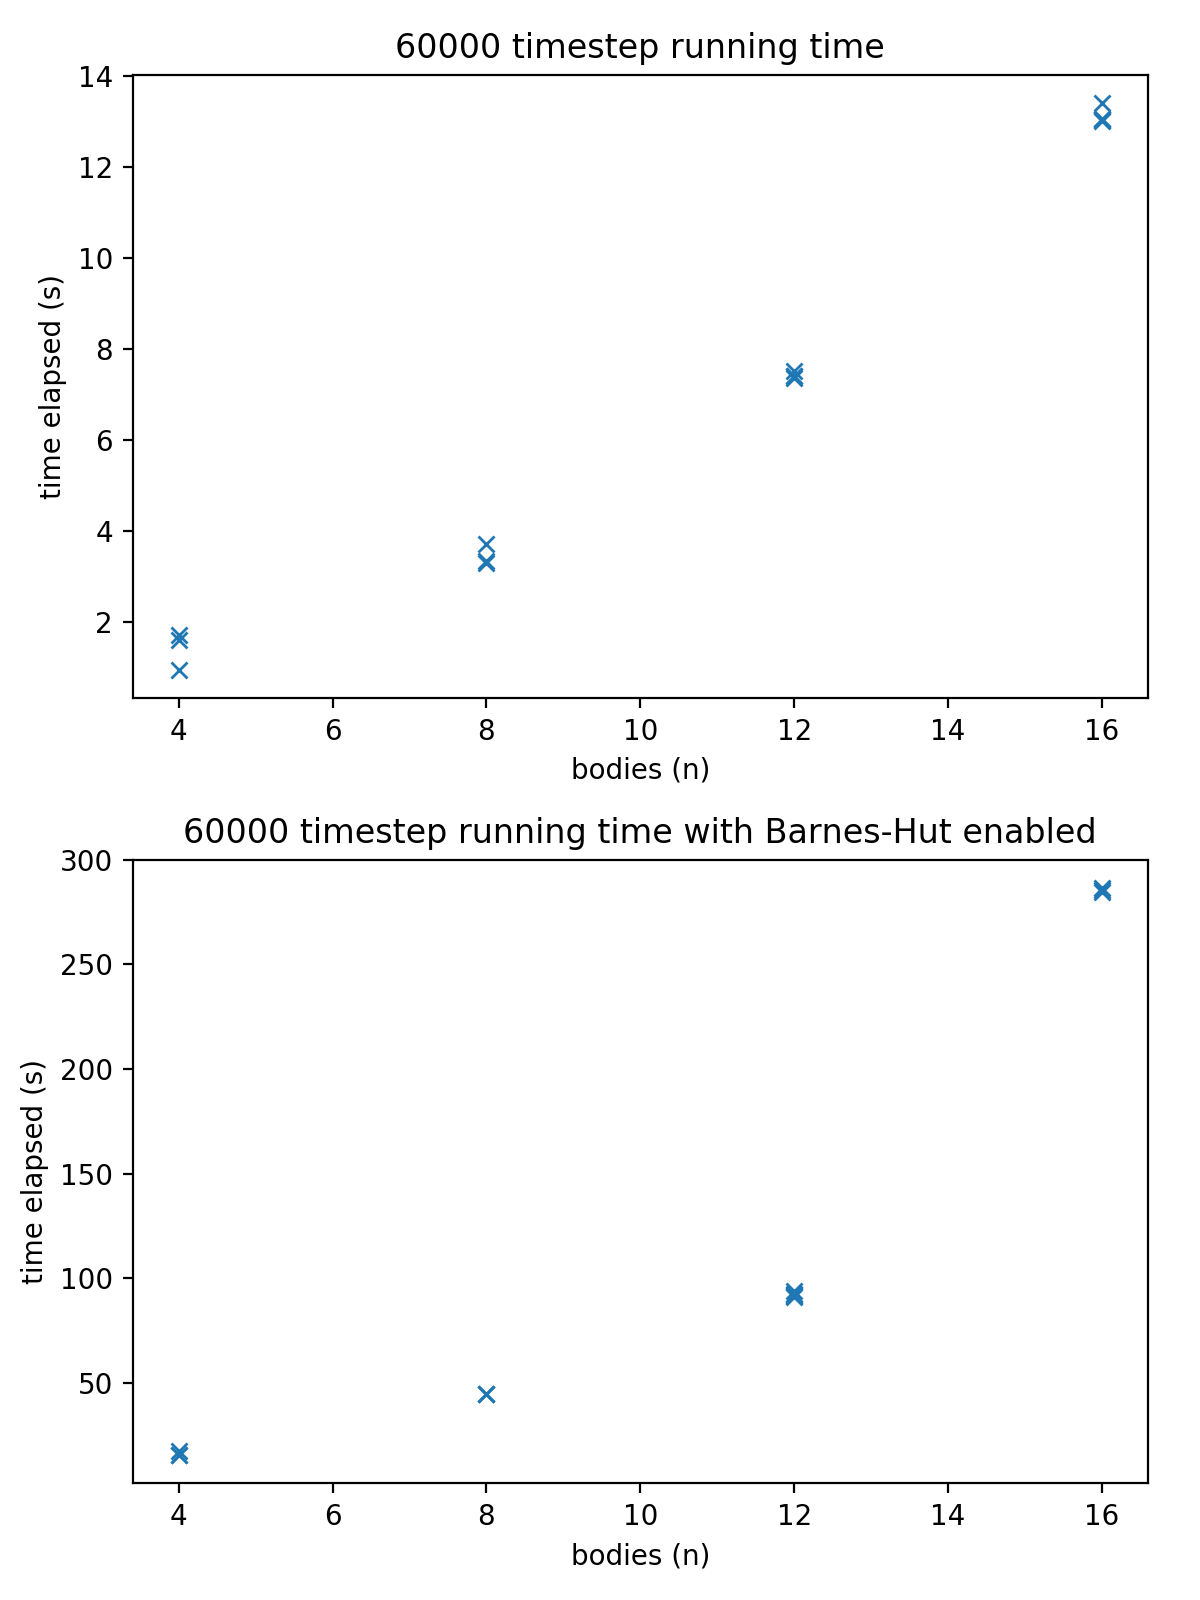
\includegraphics[width=\textwidth]{performance}
\end{figure} 

The addition of the 
\texttt{-march=native} compiler flag, which enables the use of all CPU specific instructions, provided no recognizable improvement in running time, but was left enabled in the instance that it improved performance on \texttt{goliath}.

The use of both th GCC and Clang Profile-Guided Optimisation features provided no recognizable improvement in running time.

Distressingly, \texttt{-O0}, \texttt{-O1}, \texttt{-O2}, \texttt{-O3} showed no recognizable improvement in running time. \texttt{-Ofast} led to an -4\%-ish performance regression.

By profiling with \texttt{callgrind}, we saw that execution was dominated by only one incredibly costly user-defined method, with an exclusive cost of 26.33\% of total running time.

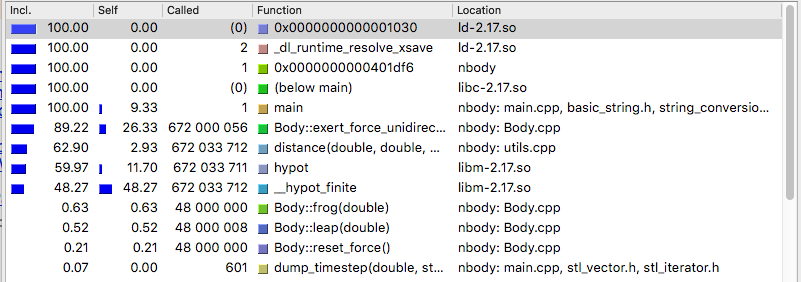
\includegraphics[width=\textwidth]{profile}

Performance fixes were divised.

\begin{verbatim}
 void Body::exert_force_unidirectionally(const Body& there) {
     const double m1 = m;
     const double m2 = there.m;

     const double delta_x = there.x - x;
     const double delta_y = there.y - y;
     
-    const double r = distance(x, y, there.x, there.y);
+    const double r = hypot(delta_x, delta_y);
-    const double r2 = r * r;
+    const double r2 = pow(r, 2);

     const double F = (G * m1 * m2) / r2;

     // turn the displacement vector between our two points into a force vector
     // of the desired magnitude
     const double scale_factor = F / r;

     Fx += delta_x * scale_factor;
     Fy += dumpsdelta_y * scale_factor;
 }
\end{verbatim}

Instead of recalculating $\Delta x$ and $\Delta y$ twice (the second time in \texttt{distance}), we calculate them only once and make a direct call to \texttt{hypot}, rather than making a call to \texttt{distance}. We also used the specialized \texttt{pow} provided by \texttt{cmath}. This yielded a recognizable 15\%ish performance improvement. 

\begin{verbatim}
diff --git a/Assignment_1/src/Body.cpp b/Assignment_1/src/Body.cpp

+void Body::exert_force_bidirectionally(Body& there) {
+    const double m1 = m;
+    const double m2 = there.m;
+
+    const double delta_x = there.x - x;
+    const double delta_y = there.y - y;
+
+    const double r = hypot(delta_x, delta_y);
+    const double r2 = pow(r, 2);
+
+    const double F = (G * m1 * m2) / r2;
+
+    // turn the displacement vector between our two points into a force vector
+    // of the desired magnitude
+    const double scale_factor = F / r;
+
+    Fx += delta_x * scale_factor;
+    Fy += delta_y * scale_factor;
+
+    there.Fx -= delta_x * scale_factor;
+    there.Fy -= delta_y * scale_factor;
+}

diff --git a/Assignment_1/src/main.cpp b/Assignment_1/src/main.cpp
@@ -258,8 +259,7 @@ int main(int argc, char **argv) {
                 for (size_t j = i + 1; j < bodies.size(); j++) {
                     auto& y = bodies[j];
-                    x.exert_force_unidirectionally(y);
-                    y.exert_force_unidirectionally(x);
+                    x.exert_force_bidirectionally(y);
                 }
             }
         }
\end{verbatim}

This fix halved execution time, for obvious reasons.\footnote{I had to throw out all my old profile data}.

\begin{verbatim}
diff --git a/Assignment_1/src/Body.cpp b/Assignment_1/src/Body.cpp
@@ -83,11 +82,11 @@ double Body::kinetic_energy() const {
 double Body::gravitational_potential_energy(const Body& there) const {
     const double R = distance(x, y, there.x, there.y); // final distance, aka, to edge

-    return (-G * m * there.m) / R;
+    return (-Gm * there.m) / R;
 }

@@ -101,7 +100,7 @@ void Body::exert_force_unidirectionally(const Body& there) {

-    const double F = (G * m1 * m2) / r2;
+    const double F = (Gm * m2) / r2;

@@ -113,7 +112,6 @@ void Body::exert_force_unidirectionally(const Body& there) {

-    const double F = (G * m1 * m2) / r2;
+    const double F = (Gm * m2) / r2;

@@ -189,6 +189,7 @@ std::vector<Body> parse_input_file(std::ifstream& input_fh) {

     for (size_t i = 0; i < bodies.size(); i++) {
         bodies[i].m = masses[i];
+        bodies[i].Gm = G * masses[i];
     }

\end{verbatim}

Precomputing $Gm$ yielded a 3\%ish performance improvement.

\section*{Parallelism}
% A description of your parallel implementation. How do you make use of OpenMP and MPI? How is information and work shared between threads and processes.  Any optimisations applied and/or challenges encountered will go here.
\subsection*{Implementation}
\subsubsection*{OpenMP}

I slapped as many \texttt{\#pragma omp parallel for shared(bodies)} on as many loops as I could find, and quickly discovered massive lock contention issues associated with \texttt{\#pragma omp critical}. Pairwise force updates between bodies:

\begin{verbatim}
    for (size_t i = 0; i < bodies.size() - 1; i++) {
        auto& x = bodies[i];
        
        for (size_t j = i + 1; j < bodies.size(); j++) {
            auto& y = bodies[j];
                x.exert_force_bidirectionally(y);
        }
    }
\end{verbatim}

where 

\begin{verbatim}
void Body::exert_force_bidirectionally(Body& there) {
    ...
    #pragma omp critical
    {
    Fx += delta_x * scale_factor;
    Fy += delta_y * scale_factor;

    there.Fx -= delta_x * scale_factor;
    there.Fy -= delta_y * scale_factor;
    }
}
\end{verbatim}

which had provided massive performance gains in the serial implementation over unidirectional updates was now causing massive parallel slowdowns, where increasing the \texttt{OMP\_NUM\_THREADS} caused a proportional increase in walltime. Instead, a \texttt{critical}-less comparison schema was devised, 

\begin{verbatim}
#pragma omp parallel for shared(bodies)
for (size_t i = 0; i < bodies.size(); i++) {
    auto& x = bodies[i];

    for (size_t j = 0; j < bodies.size(); j++) {
        auto& y = bodies[j];

        if (&bodies[i] != &bodies[j]) {
            // XXX: Do NOT swap these around. You will cause
            // race conditions
            x.exert_force_unidirectionally(y);
        }
    }
}
\end{verbatim}

that provided the sought after parallel speedup. This parallel speedup was found to be present at where $n$-bodies was high. Testing focussed primarily on $n > 5000$,\footnote{In MS1, I failed to test simulations with a large number of $n$, as I was focussed on testing the accuracy of the implementation, and generated input files would cause high numbers of collisions that made accuracy assessment difficult. Testing $n=10000$, we find a 10x speedup with by using a serial Barnes-Hut implementation (Avg. $1.12$s, as opposed to $9.87$s without Barnes-Hut). Barnes-Hut afforded a much simpler parallelization scheme, as each body could calculate its force against the quadtree concurrently, without locks} where force and integration calculation overhead dominated thread creation overhead. Parallel speedup vanished around the $n \approx 500$ mark.

% Increasing \texttt{OMP_NUM_THREADS} beyond \texttt{4} failed to provide a speedup at $n = 10000$.

\subsubsection*{MPI}

Looking at our high-level implementation, the following two steps consume the vast majority of our computing power:

\begin{enumerate}
    \item Inserted all \texttt{Body}s into a fresh \texttt{QuadTree} on full timesteps, traversing the \texttt{QuadTree} with every \texttt{Body} to calculate forces ($O(n \log n)$)
    \item Performed the appropriate \textit{Leapfrog} step to derive new velocities \textit{or} positions
\end{enumerate}

The \textit{Leapfrog} step is the easiest step to distribute amongst many nodes, as it does not require the comparison of a body to all other bodies - each node can compute the step on a subset of all bodies, and later combine each subset with relatively simple MPI code.

This can be achieved with \texttt{MPI\_Scatterv} and \texttt{MPI\_Gatherv}
\footnote{These \texttt{v} variants support custom chunking sizes e.g. if we have 15 bodies we can send $4, 4, 4, 3$ bodies to each node respectively, which \texttt{MPI\_Scatter} and \texttt{MPI\_Gather} do not support dynamic chunking}. We decompose each dimension of our \texttt{Body}s into arrays, (e.g. the $x$ position, the $x$ veolocity, etc.), \texttt{MPI\_Scatterv} these arrays, recompose them into \texttt{Body}s, run \texttt{Leapfrog} on this subset on each node, decompose the subset into arrays, \texttt{MPI\_Gatherv} these arrays back to the root node, and recompose them into $\texttt{Bodys}$.

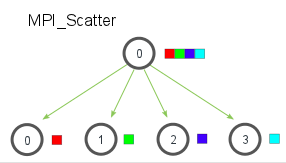
\includegraphics[width=7cm]{mpi_scatter}
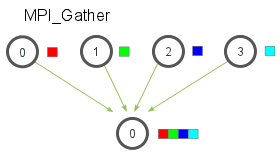
\includegraphics[width=7cm]{mpi_gather}

\begin{verbatim}
std::vector<Body> sbodies = scatter_bodies(bodies, size, rank);

#pragma omp parallel for shared(bodies)
for (size_t i = 0; i < sbodies.size(); i++) {
    auto& body = sbodies[i];

    if (step % 2 == LEAP) {
        body.leap(timestep);
    }
    else {
        body.frog(timestep);
    }
}

bodies = gather_bodies(sbodies, size, rank, bodies.size());
\end{verbatim}

where \texttt{sbodies} is our subset of bodies distributed to each node. 

Because force calculation is only performed on the root node, this messaging architecture is \textit{master-slave}, where the root node coordinates gathers and scatters. Slave nodes, are, unfortunately, underutilized. Further work could be sent distributing force calculation work, doing away with a root node entirely, except for logging.

\begin{verbatim}
Total CPU time on rank 0 was 89.820000
Total CPU time on rank 2 was 36.750000
Total CPU time on rank 3 was 36.960000
Total CPU time on rank 1 was 37.040000
\end{verbatim}


% A description of how you have verified the correctness of your parallel implementation. (See comments for MS1)
\subsection*{Verification \& Correctness}

Because of my confidence in the correctness of the serial implementation, it served as a reference implementation for the verification of the parallel implementation.

Both implementations were run with identical input parameters, and their outputs were \texttt{diff}d. When run without MPI enabled, outputs were identical. When run with MPI, floating point abnormalities (initially affecting the least significant digits of each floating point value) gradually caused each diff to diverge. I hypothesize that the MPI serialization and deserialization procedure was truncating precision and causing this divergence. Perhaps some option exists to ensure that MPI guarantees floating point precision.


% A credible plan of jobs to run to measure the scalability of your parallel implementation. The idea here is that you could take this plan an start performing timing experiments. You should not organise your testing so that if your test plan is curtailed, then you can still draw sensible conclusions from the results you do get.
\subsection*{Scalability}

We have mulitple dimensions that we can change to measure the scalability of the parallel implementation.

\begin{enumerate}
    \item The number of bodies ($n$) (\texttt{512, 1024, 2048, 4096, 8192, 16384})
    \item \texttt{ENABLE\_BARNES\_HUT} (\texttt{true, false})
    \item \texttt{--nodes} (\texttt{Disabled, 1, 4, 16})
    \item \texttt{--ntasks} (\texttt{1, 4, 16})
    \item \texttt{--ntasks-per-node} (\texttt{1, 4})
    \item \texttt{--cpus-per-task} (\texttt{1, 4, 16})
    \item \texttt{\#pragma omp parallel schedule(static, dynamic, guided)}
\end{enumerate}

Running tests with all valid combinations of these variables, with a \texttt{numTimeSteps} as low as 8, would produce useful data, across multiple dimension, with minimal load on cluster. It would be unlikely that this plan would be curtailed.

\medskip

\bibliographystyle{ieeetr}
\bibliography{bib}

\end{document}
